\chapter{Laboratory Data}
\label{appendix:Lab data}
In this appendix the laboratory data will be illustrated in detail. Here, one can find all the results and Figure corresponding to the data which is referred to in the report.
\section{Bed Load Samples}
The bed load samples collected were all weighed before they were put in the oven. 
There are 7 samples collected at 4 different locations. The first three locations are the cross sections around the extracting point in the bifurcation of the Rio Parana Guazu with the Rio Talabera. For these three cross sections two samples were taken from the soil, one at 10 meters depth and one at 14-15 meters depth. 
The last sample was taken at 10 meters of depth in the cross section upstream close to the Puerto Ibicuy.

The Figure below shows all the samples on the weighing scale before they were put in the oven as shown in chapter 4 \ref{chap:methodology}. 

\section{Recapitulatory Table}
In this table, the details about the samples can be found for all cross sections.

\begin{table}[h]
\centering
\caption{Measurement of Saturated and Dry Weights for Samples}
\label{tab:weights}
\begin{tabular}{l S[table-format=5.2] S[table-format=5.2] S[table-format=5.2]}
\toprule
\textbf{Sample} & \textbf{Saturated Weight (g)} & \textbf{Dry Weight (g)} & \textbf{Weight of tray (g)}\\
\midrule
1-1 & 400.4 & 282.1 & 88.4\\
1-2 & 360.1 & 320,8 & 109.0 \\
2-1 & 410.1 & 317.6 & 117.1\\
2-2 & 454.9 & 404.0 & 92.5\\
3-1-A & 365.8 & 285.3 & 106.7 \\
3-1-B & 332.2 & 248.2 & 101.5 \\
3-2 & 527.8 &  368.8 & 99.1 \\
4-1 & 507.0 & 332.1 & 89.7\\
\bottomrule
\end{tabular}
\end{table}

\clearpage
\section{Bed Load Samples Pictures}
Therefore, the figures of the samples on the weighting scale are included as references.

\begin{figure}[H]
    \centering
    % First row of subfigures
    \begin{subfigure}[b]{0.48\textwidth}
        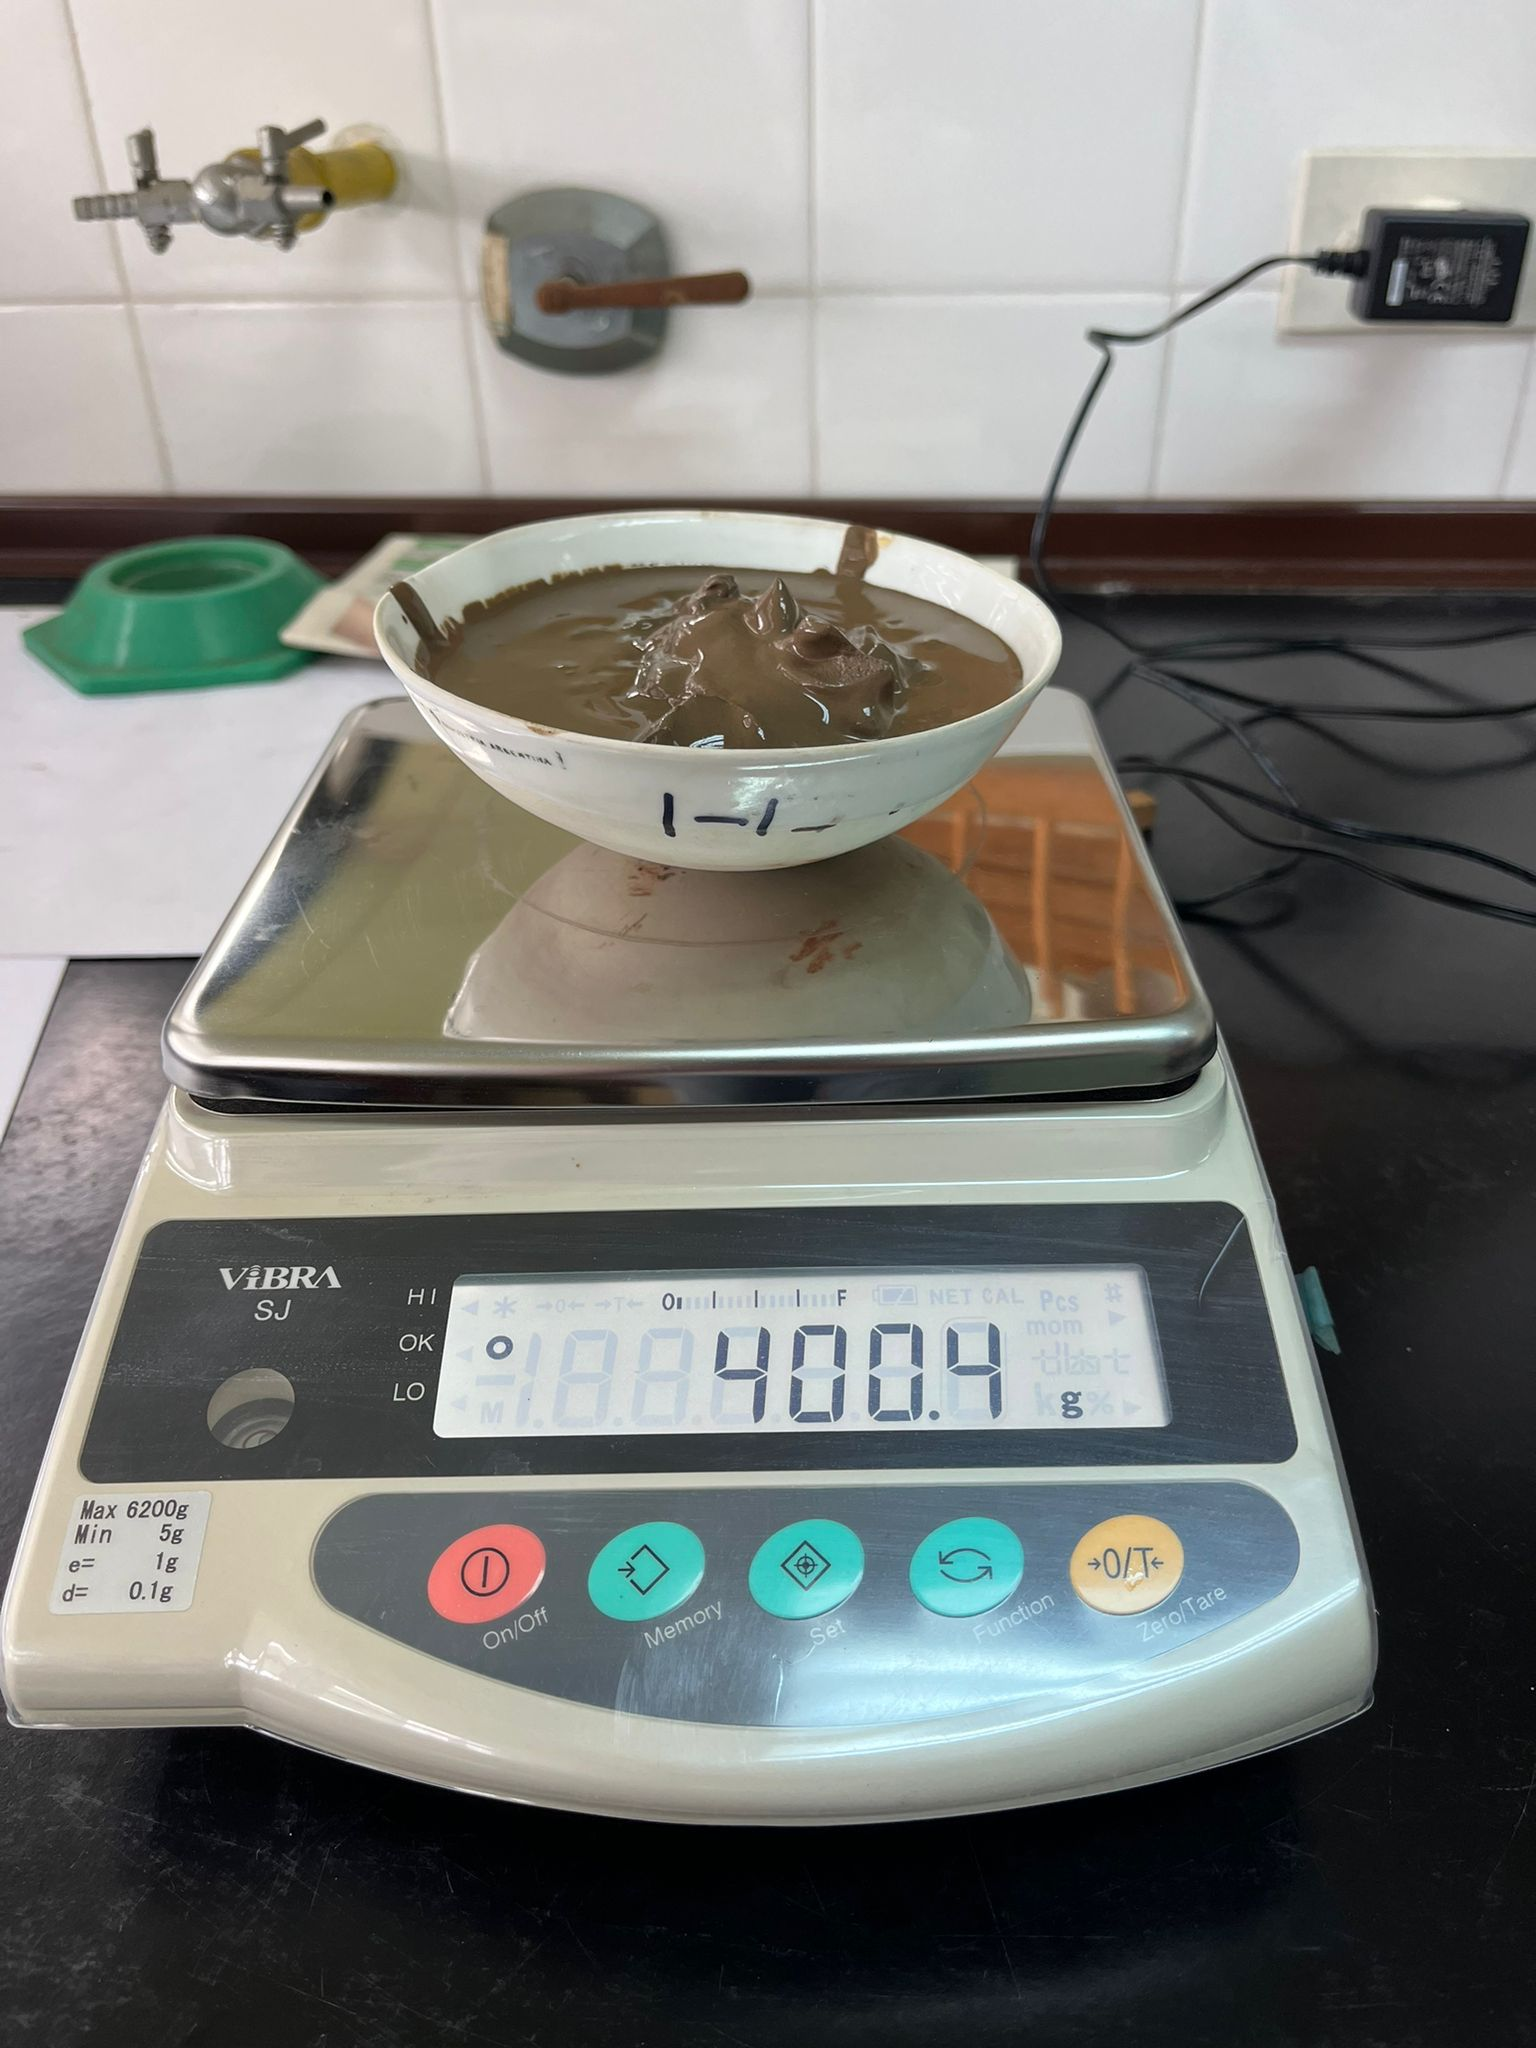
\includegraphics[width=\linewidth, height =9cm]{figures/appendix-f/1-1.jpg}
        \caption{Sample 1-1}
        \label{fig:second}
    \end{subfigure}
    \hfill
    \begin{subfigure}[b]{0.48\textwidth}
        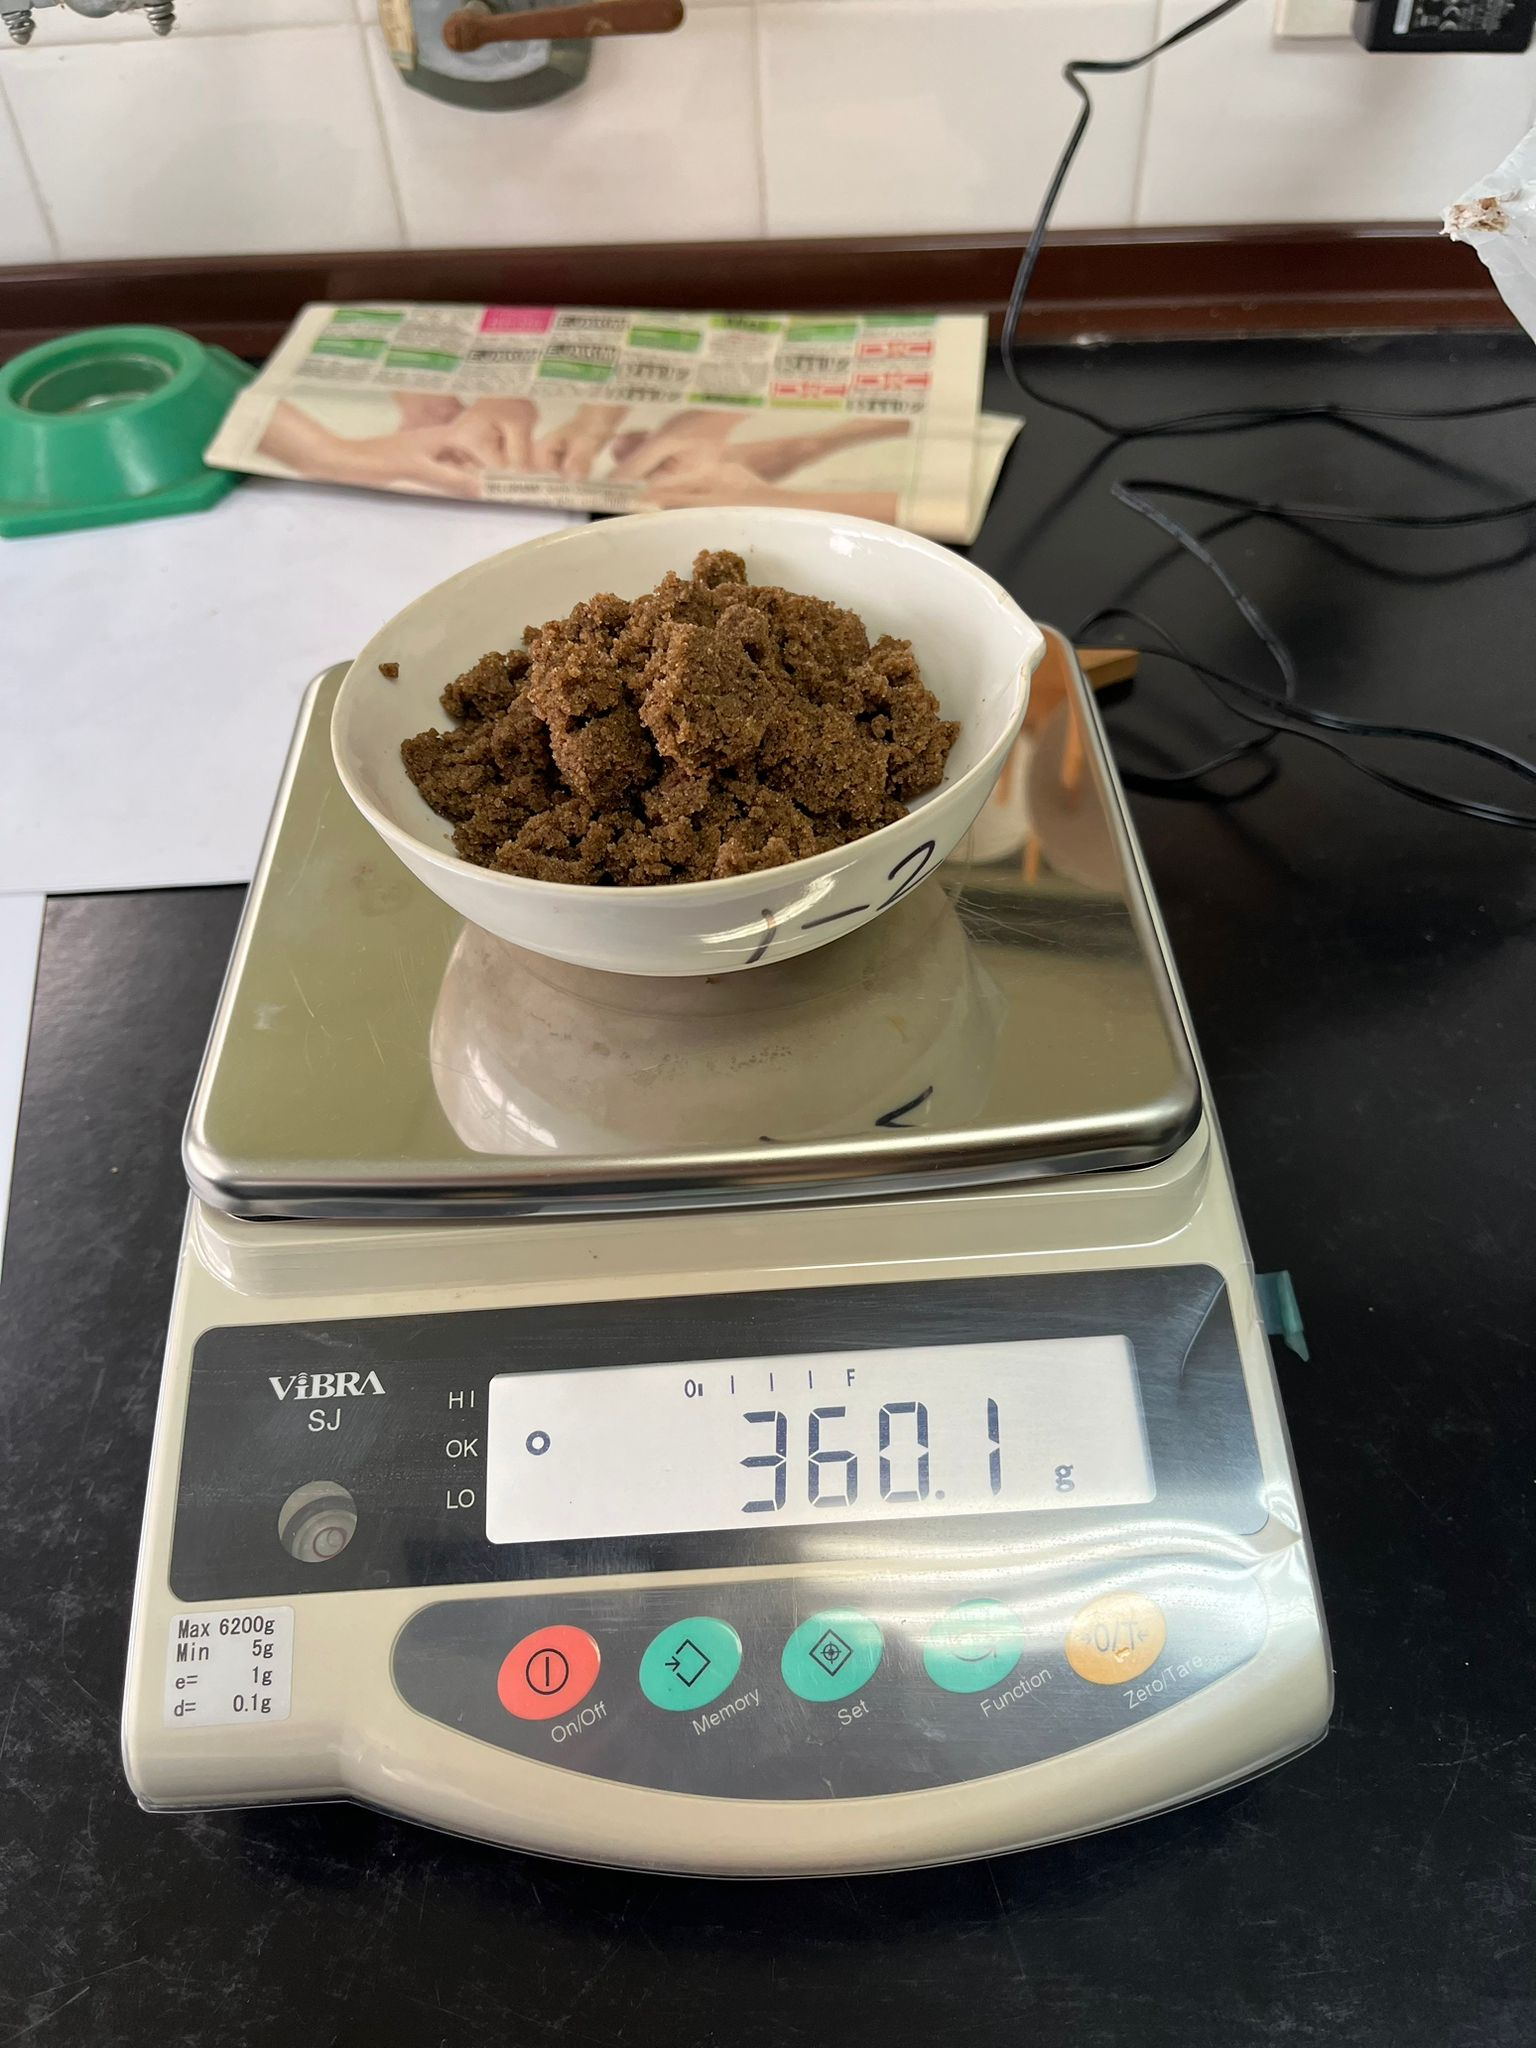
\includegraphics[width=\linewidth, height =9cm]{figures/appendix-f/1-2.jpg}
        \caption{Sample 1-2}
        \label{fig:second}
    \end{subfigure}
    

    % Second row of subfigures (add some vertical space)
    \vspace{0.5cm}

    % Second row of subfigures
    \begin{subfigure}[b]{0.48\textwidth}
        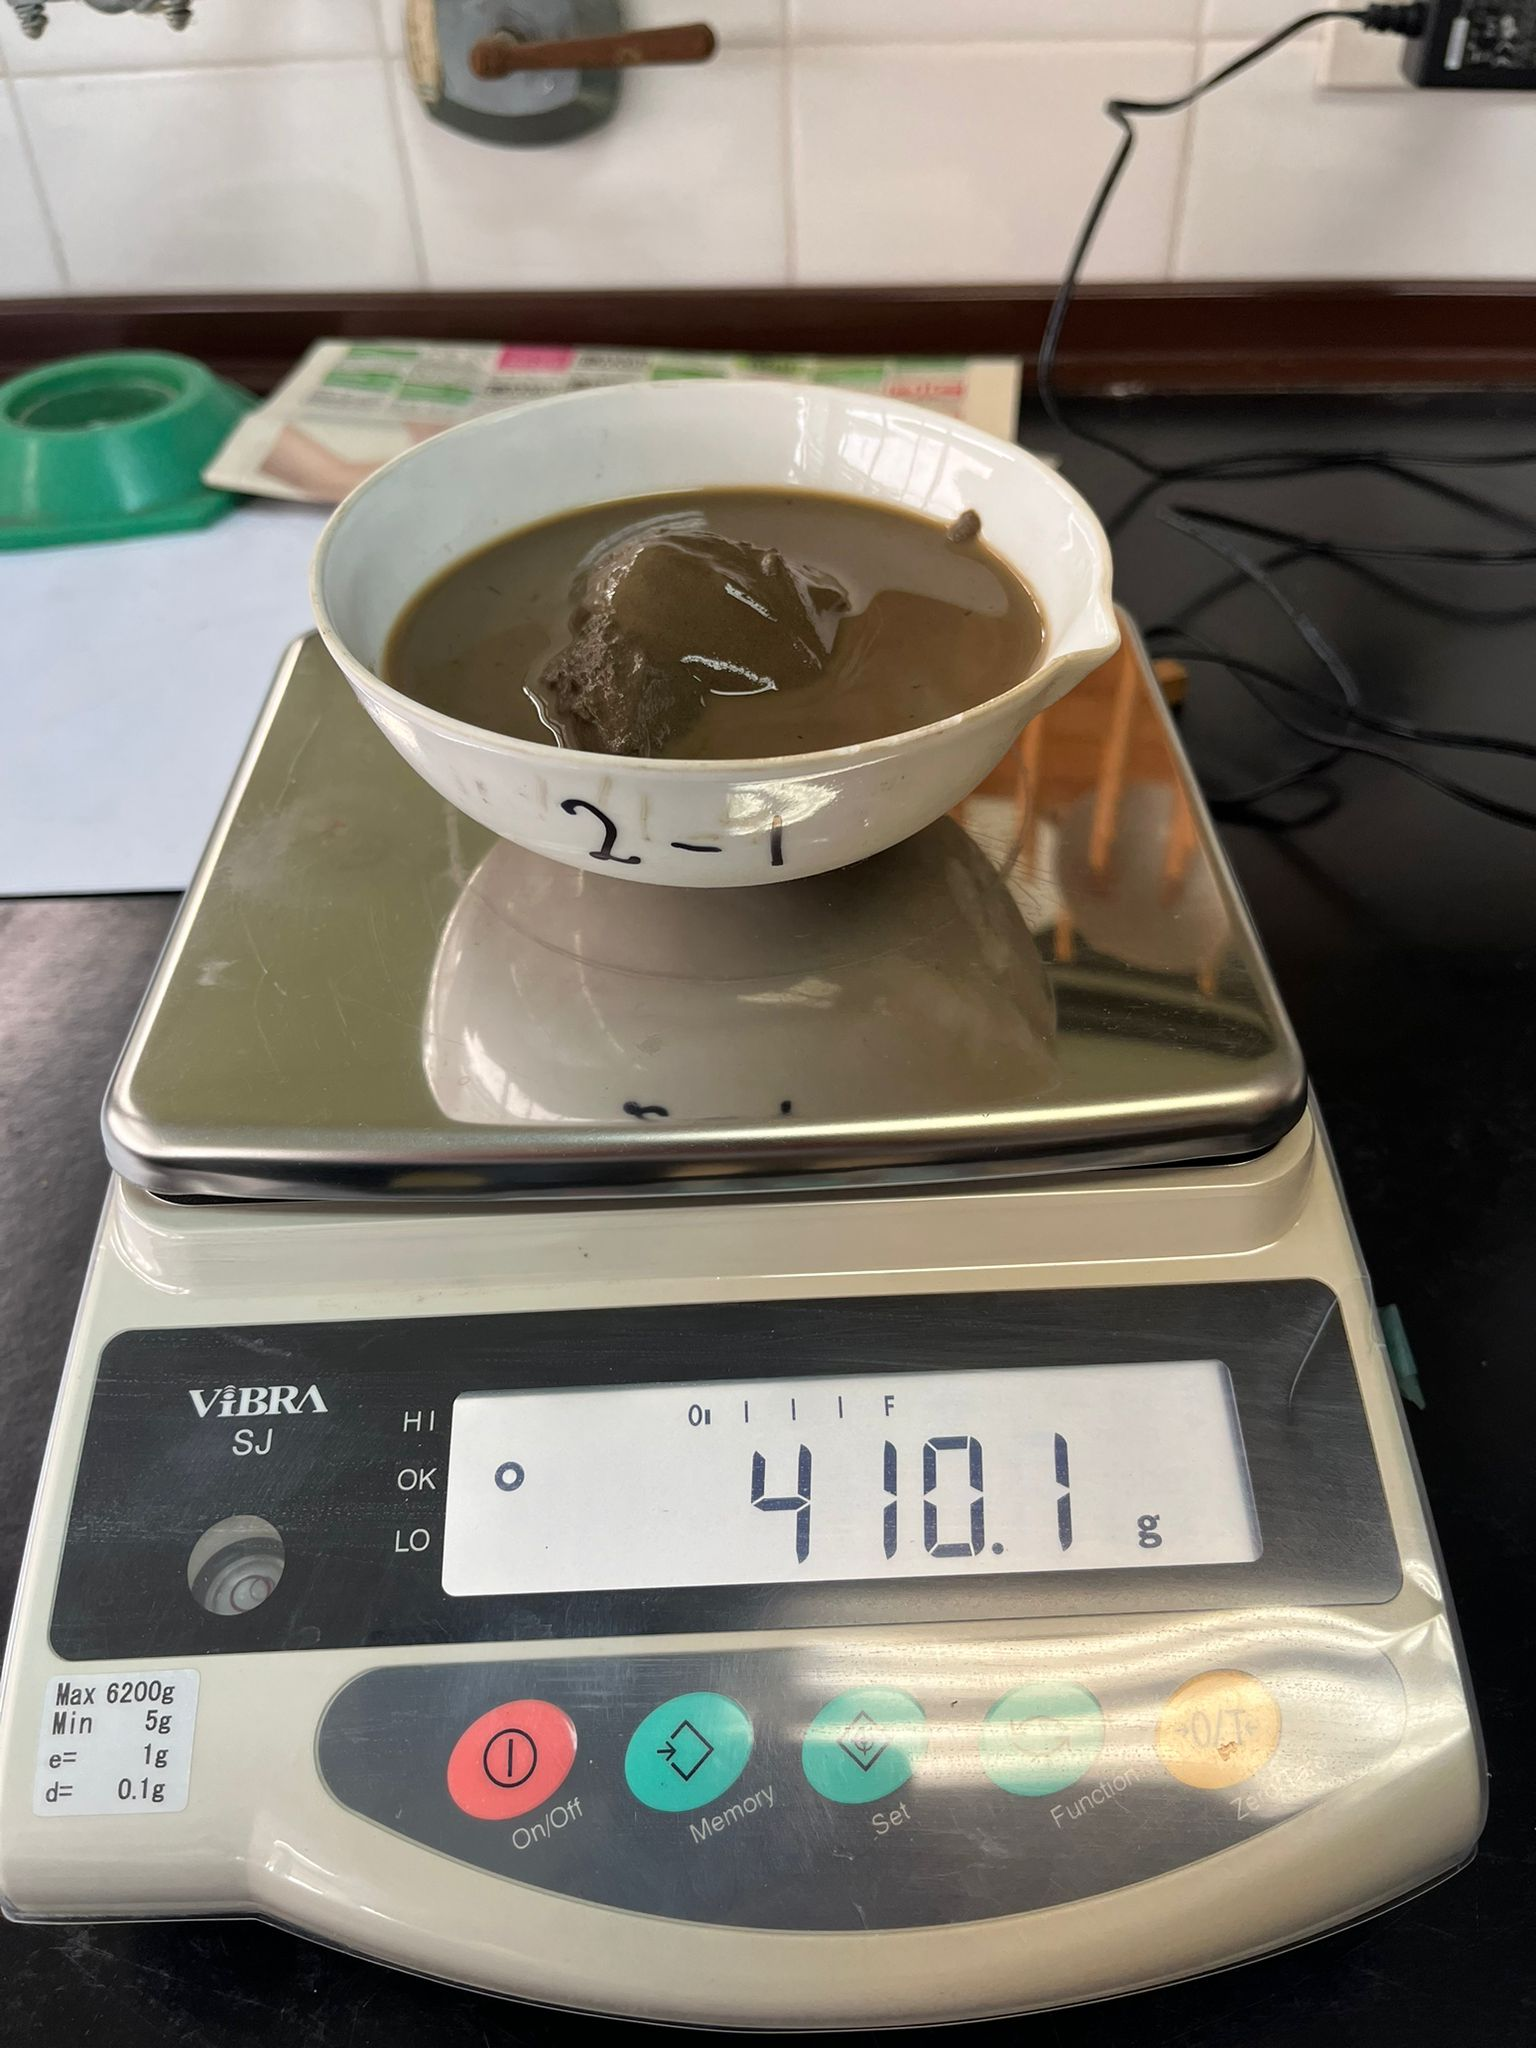
\includegraphics[width=\linewidth, height =9cm]{figures/appendix-f/2-1.jpg}
        \caption{Sample 2-1}
        \label{fig:second}
    \end{subfigure}
    \hfill
    \begin{subfigure}[b]{0.48\textwidth}
        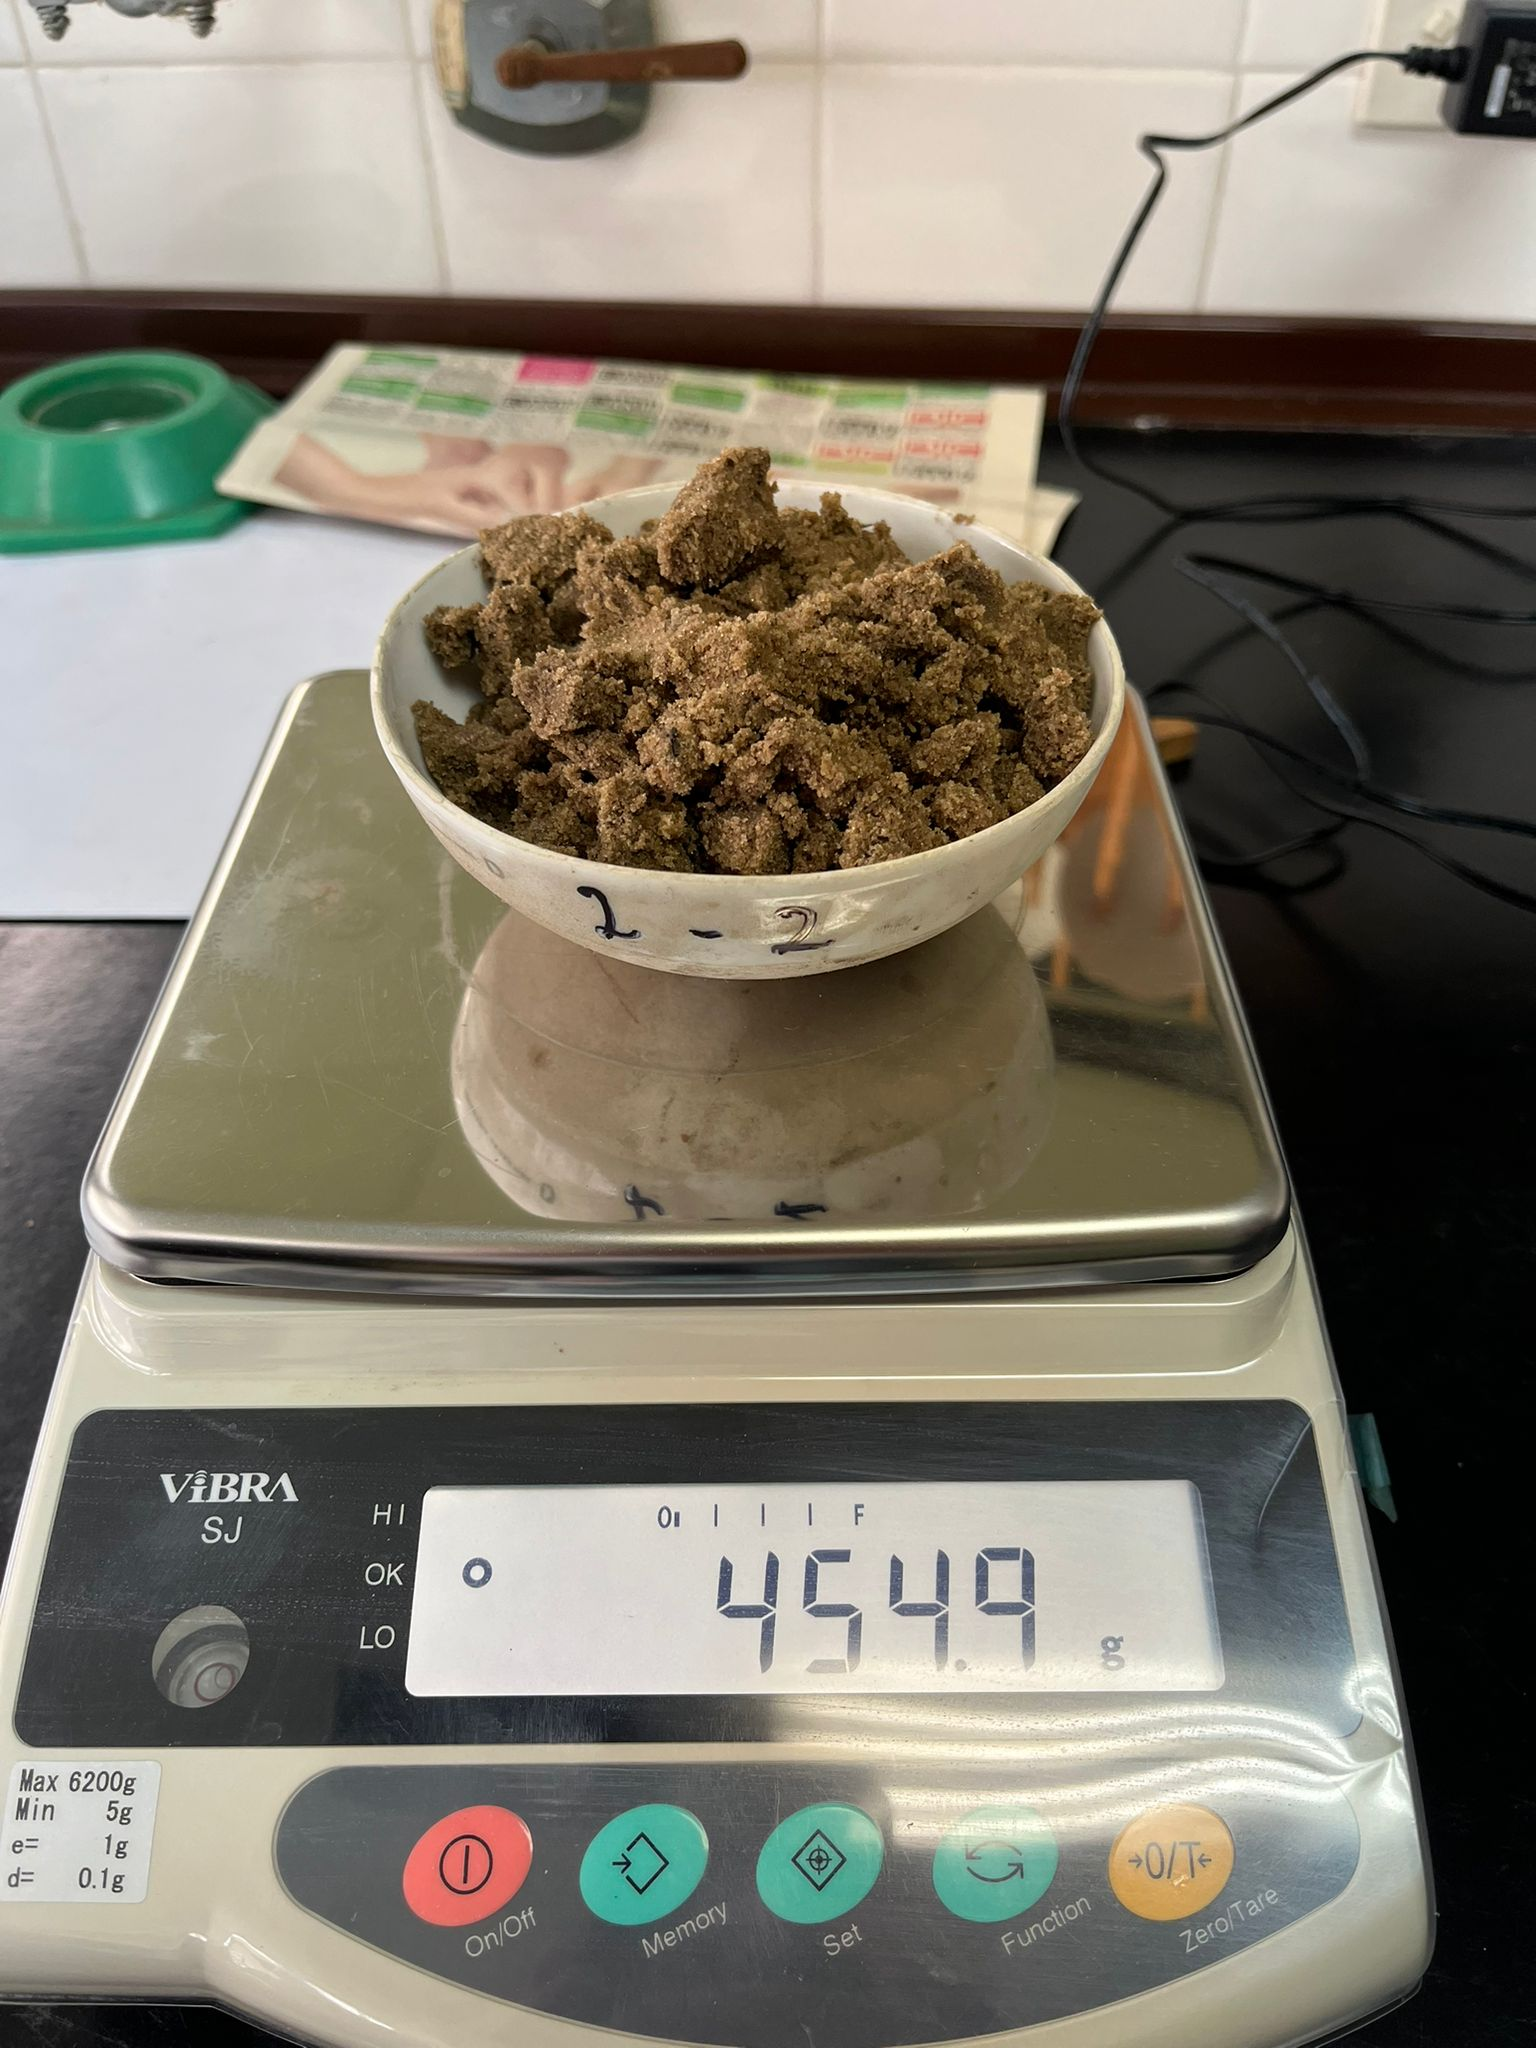
\includegraphics[width=\linewidth, height =9cm]{figures/appendix-f/2-2.jpg}
        \caption{Sample 2-2}
        \label{fig:second}
    \end{subfigure}

    \caption{Samples from Bed Load Part 1}
    \label{fig:all four 1}
\end{figure}
\clearpage
On the following page, one can find the second part of the samples from the bed load.

\begin{figure}[H]
    \centering
    % First row of subfigures
    \begin{subfigure}[b]{0.48\textwidth}
        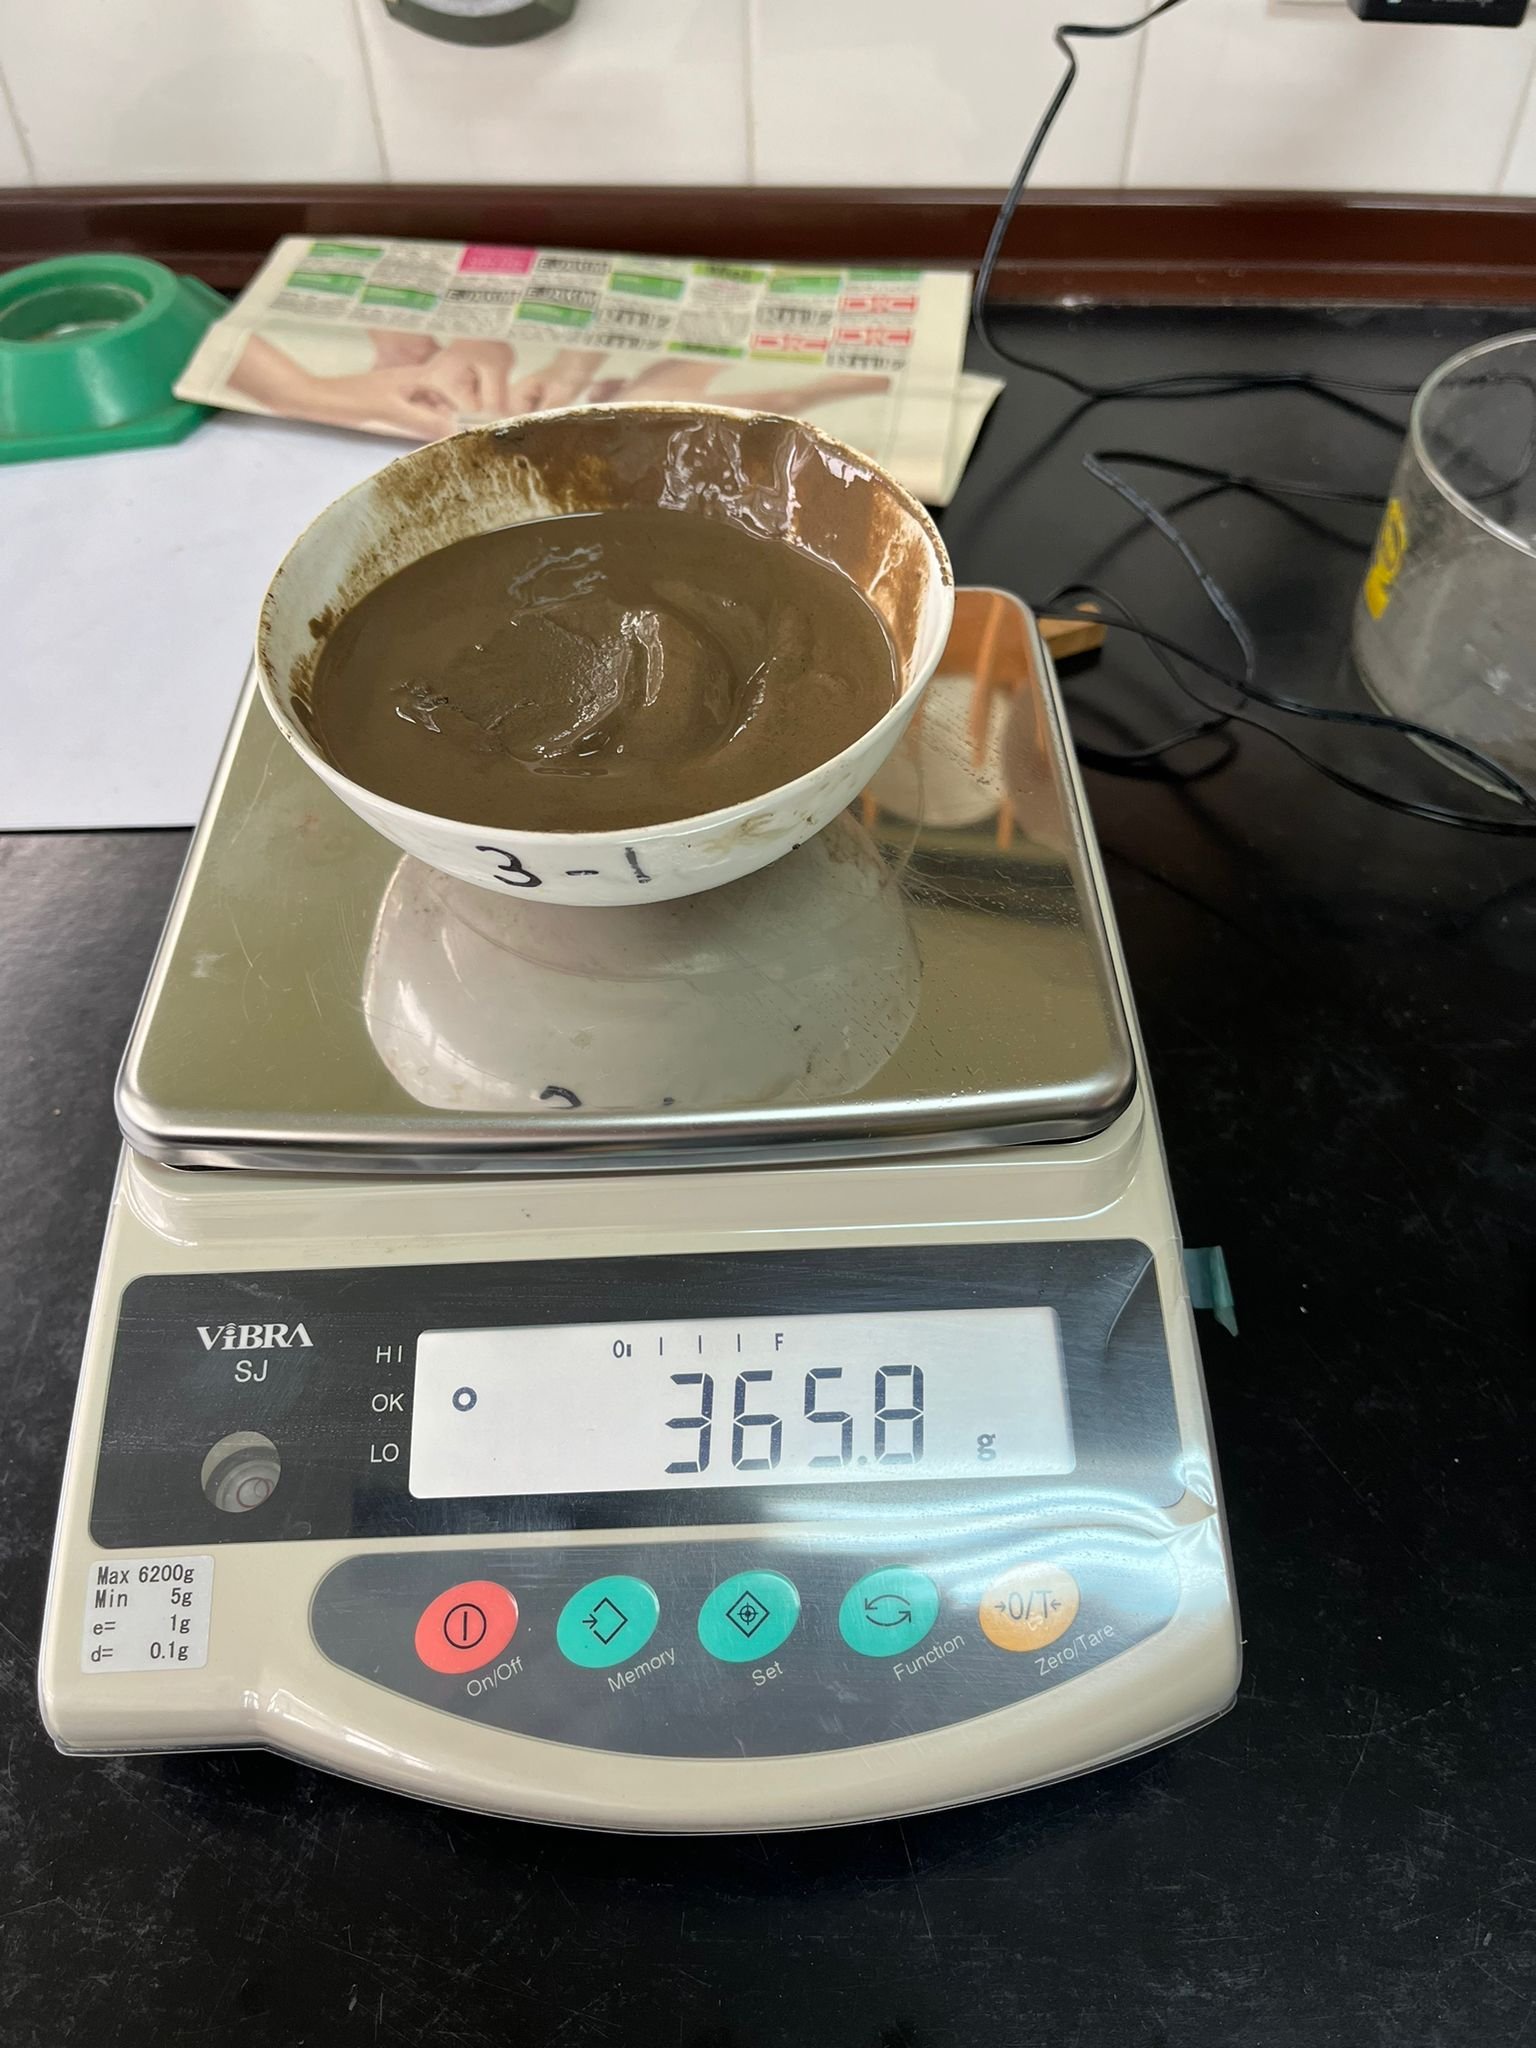
\includegraphics[width=\linewidth, height =9cm]{figures/appendix-f/3-1-A.jpg}
        \caption{Sample 3-1-A}
        \label{fig:second}
    \end{subfigure}
    \hfill
    \begin{subfigure}[b]{0.48\textwidth}
        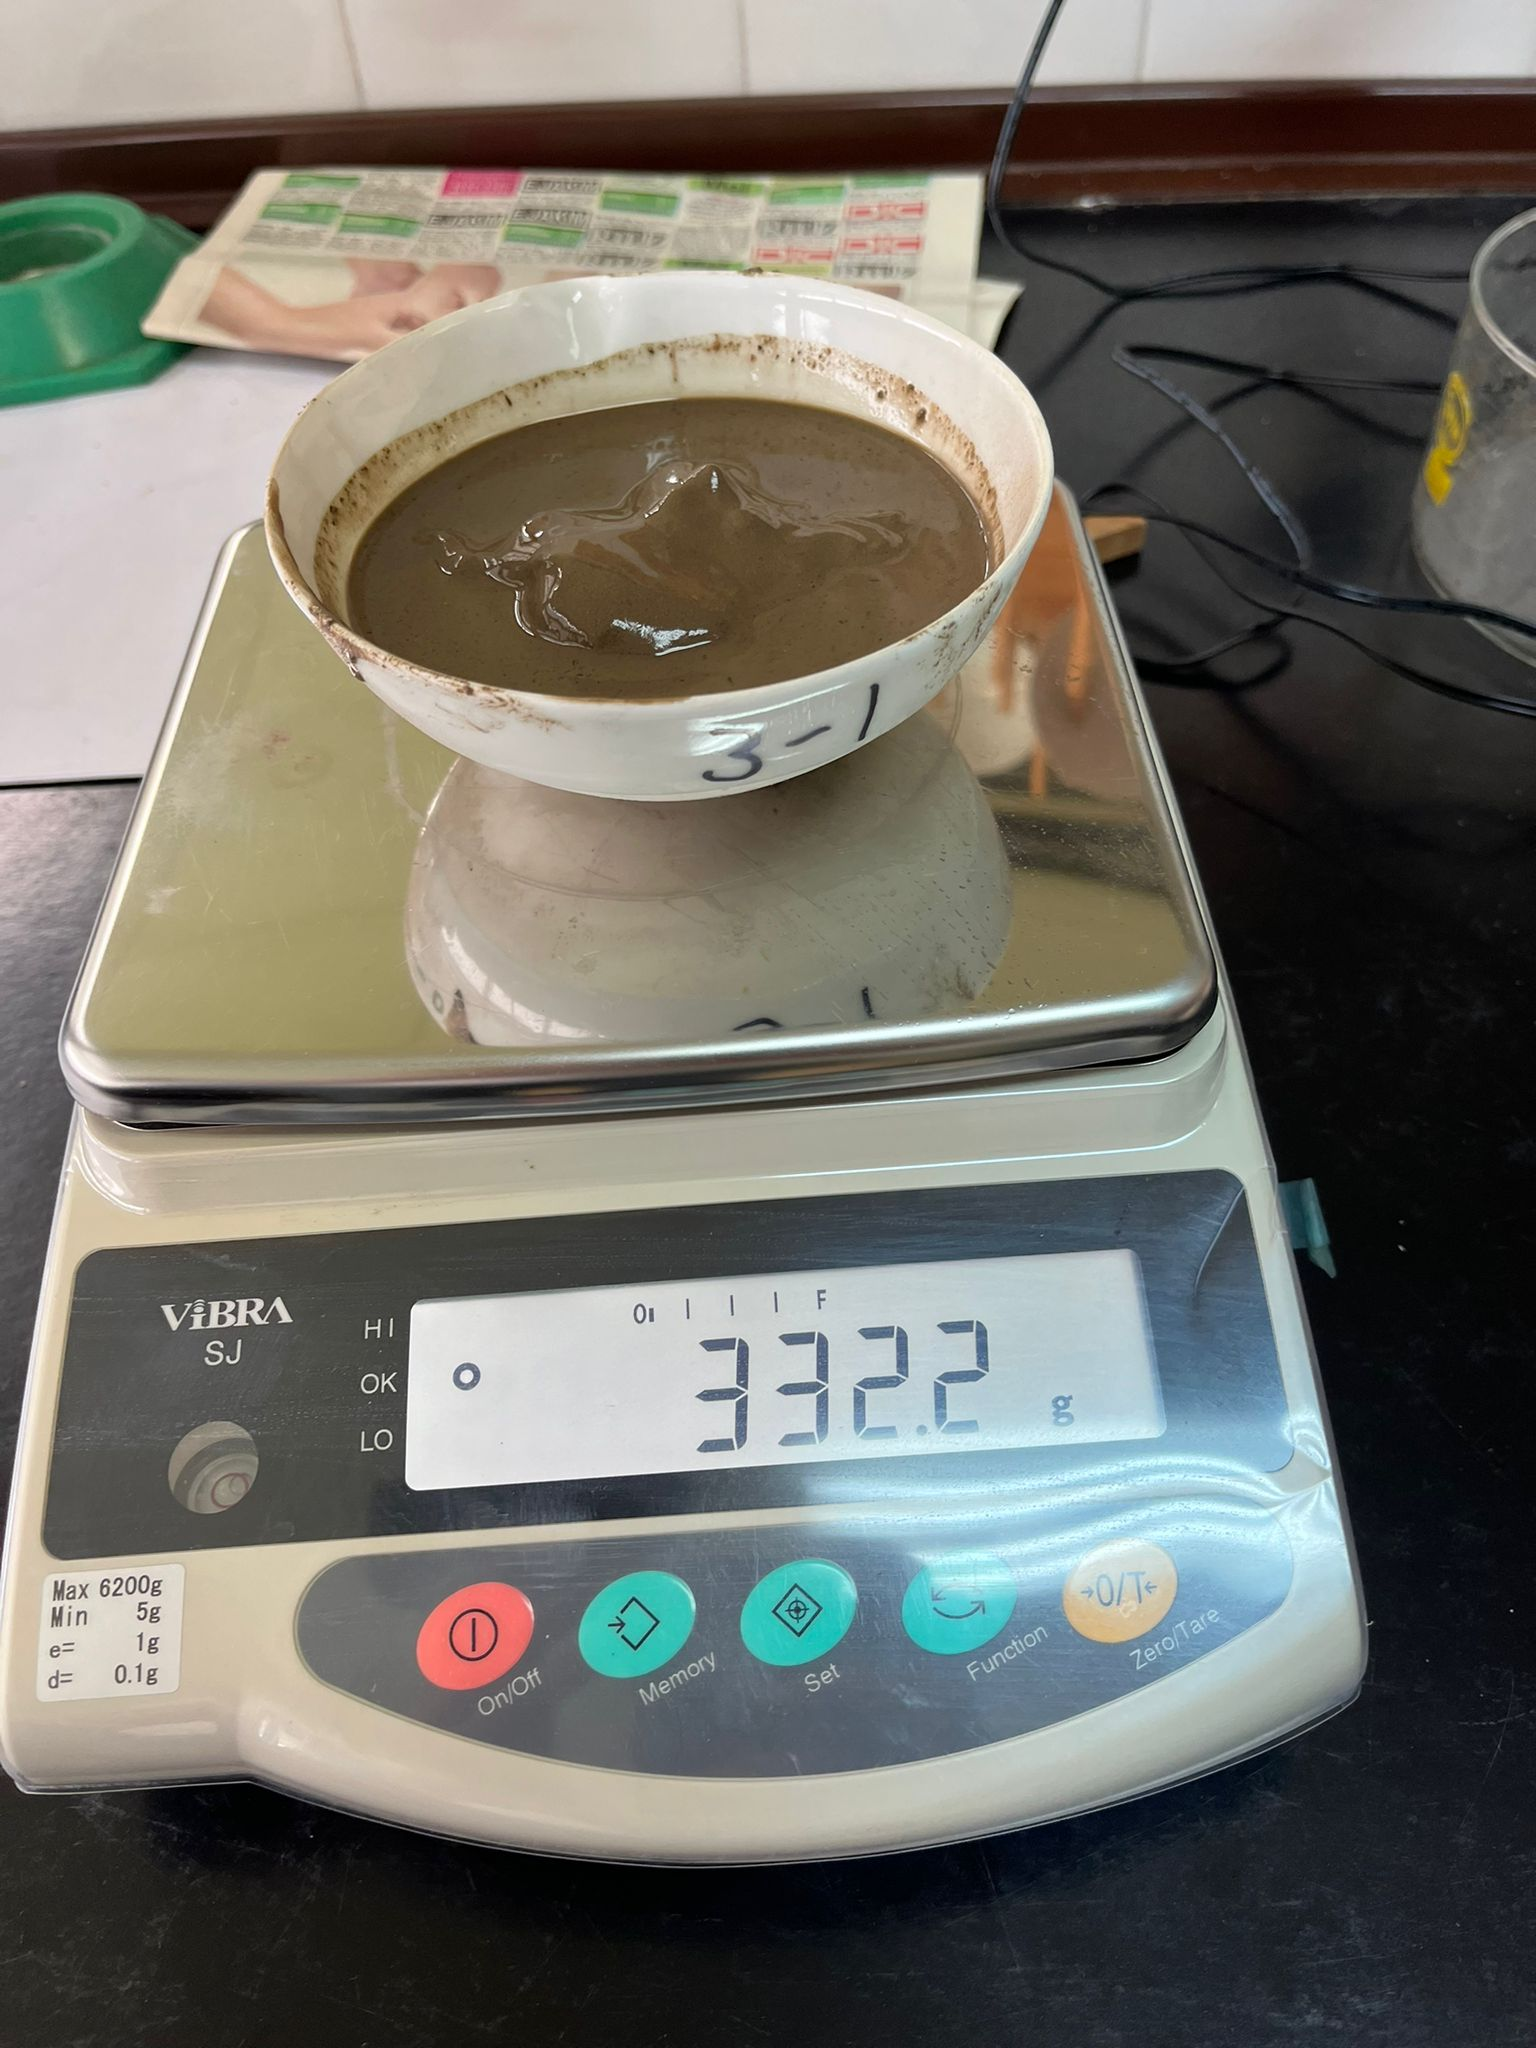
\includegraphics[width=\linewidth, height =9cm]{figures/appendix-f/3-1-B.jpg}
        \caption{Sample 3-1-B}
        \label{fig:second}
    \end{subfigure}
    

    % Second row of subfigures (add some vertical space)
    \vspace{0.5cm}

    % Second row of subfigures
    \begin{subfigure}[b]{0.48\textwidth}
        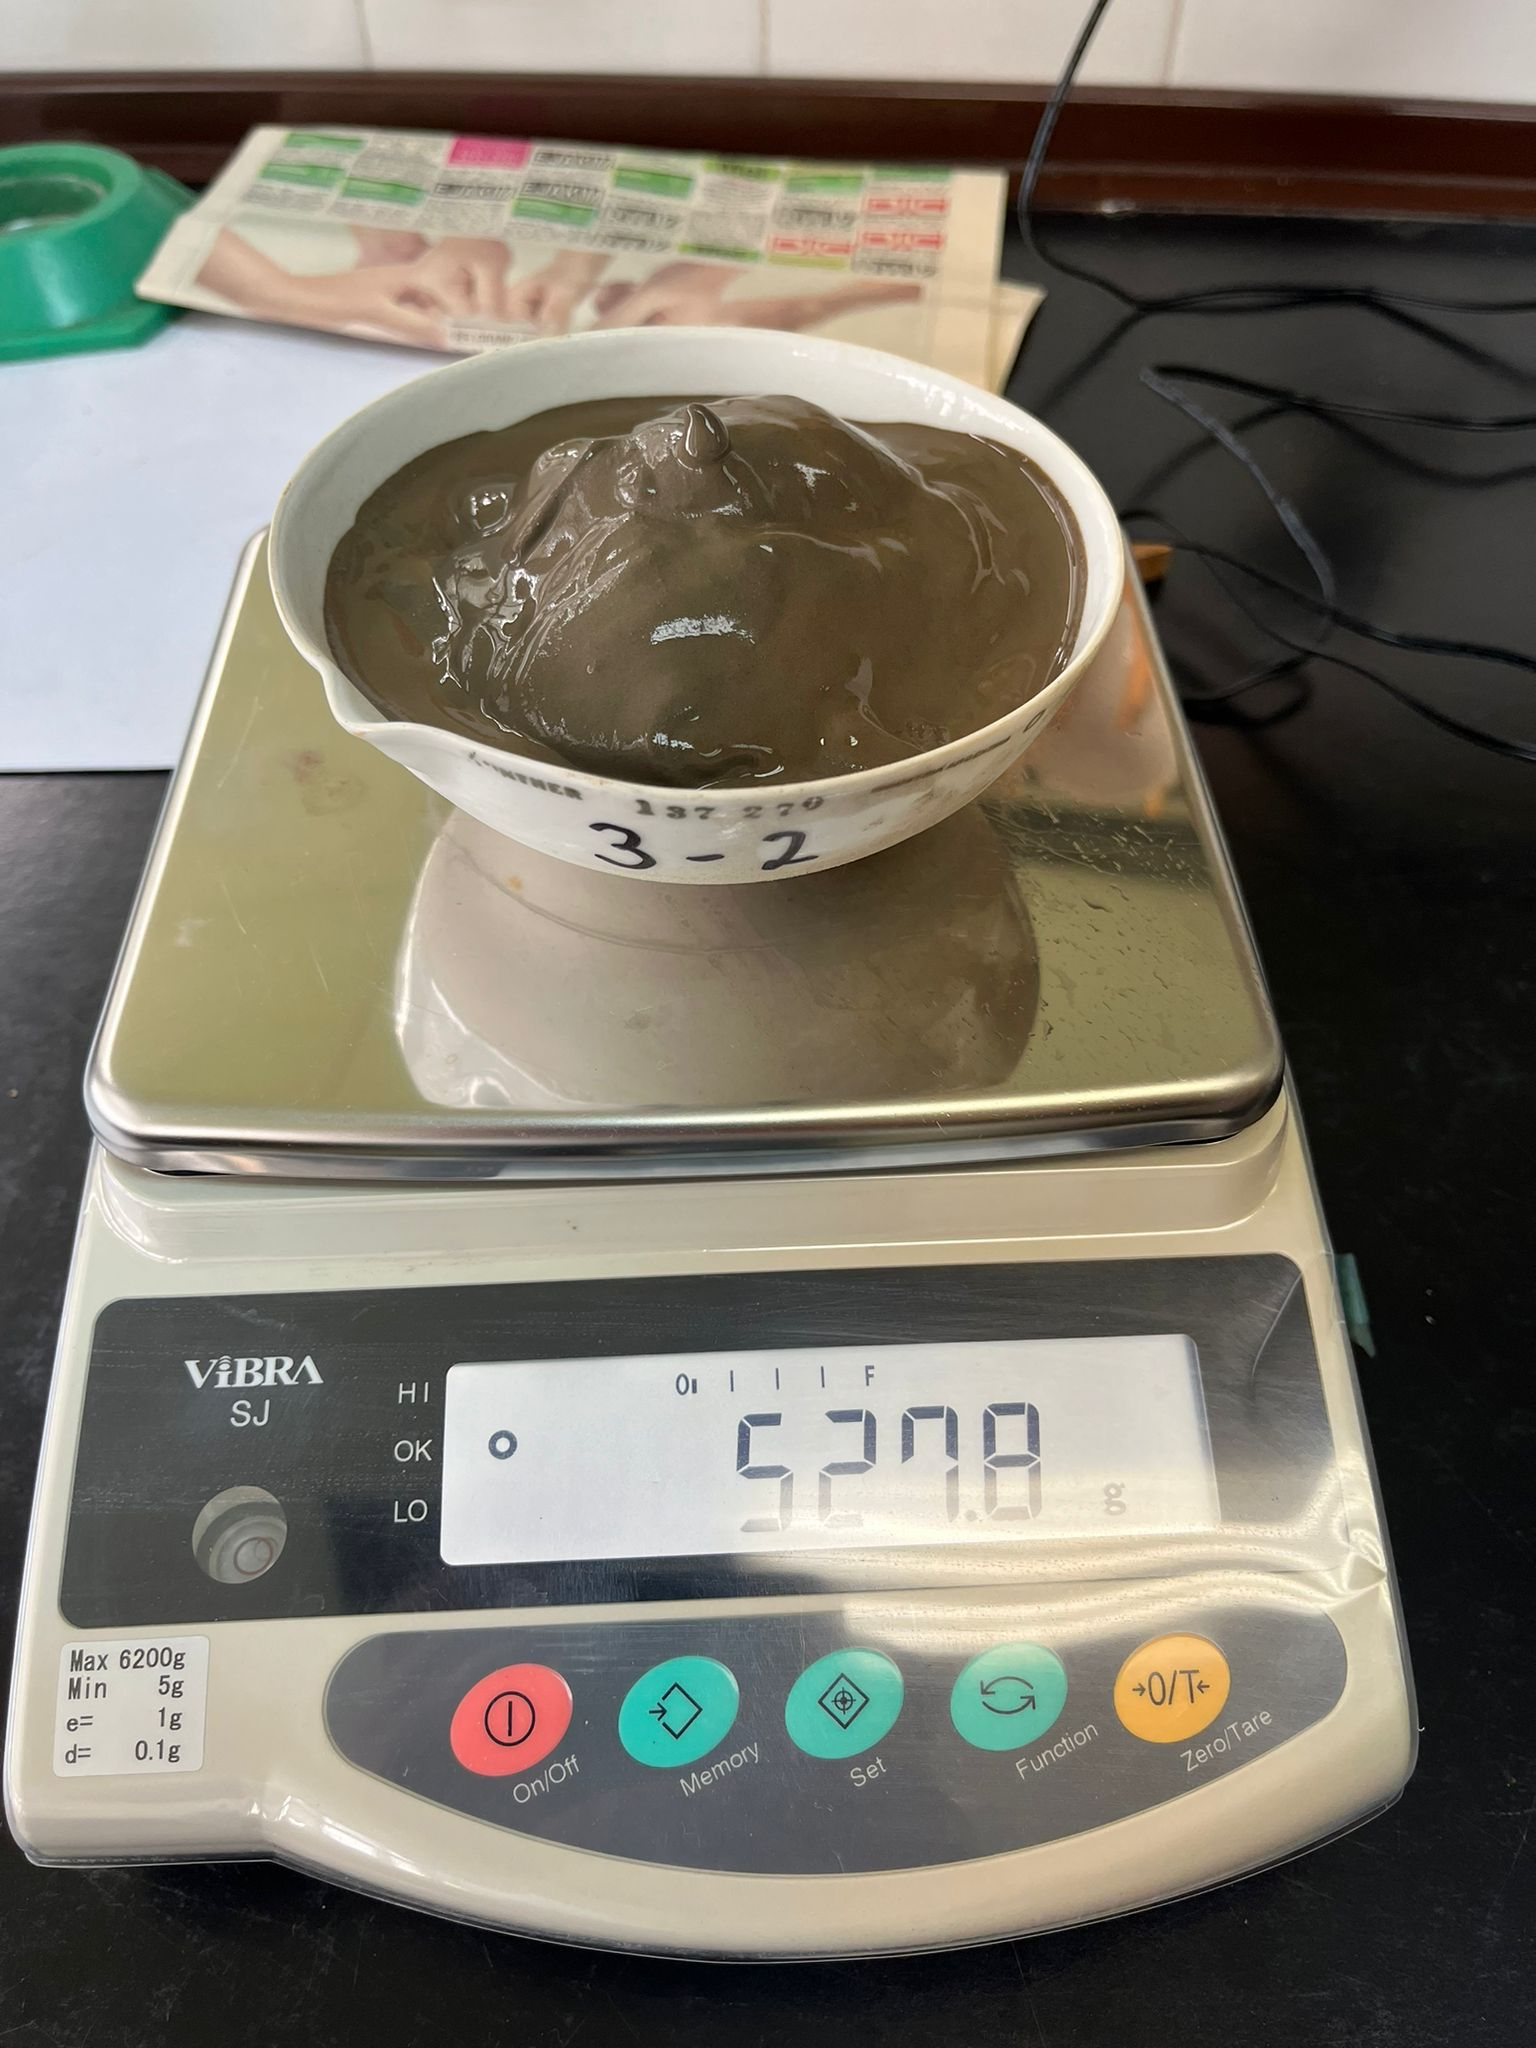
\includegraphics[width=\linewidth, height =9cm]{figures/appendix-f/3-2.jpg}
        \caption{Sample 3-2}
        \label{fig:second}
    \end{subfigure}
    \hfill
    \begin{subfigure}[b]{0.48\textwidth}
        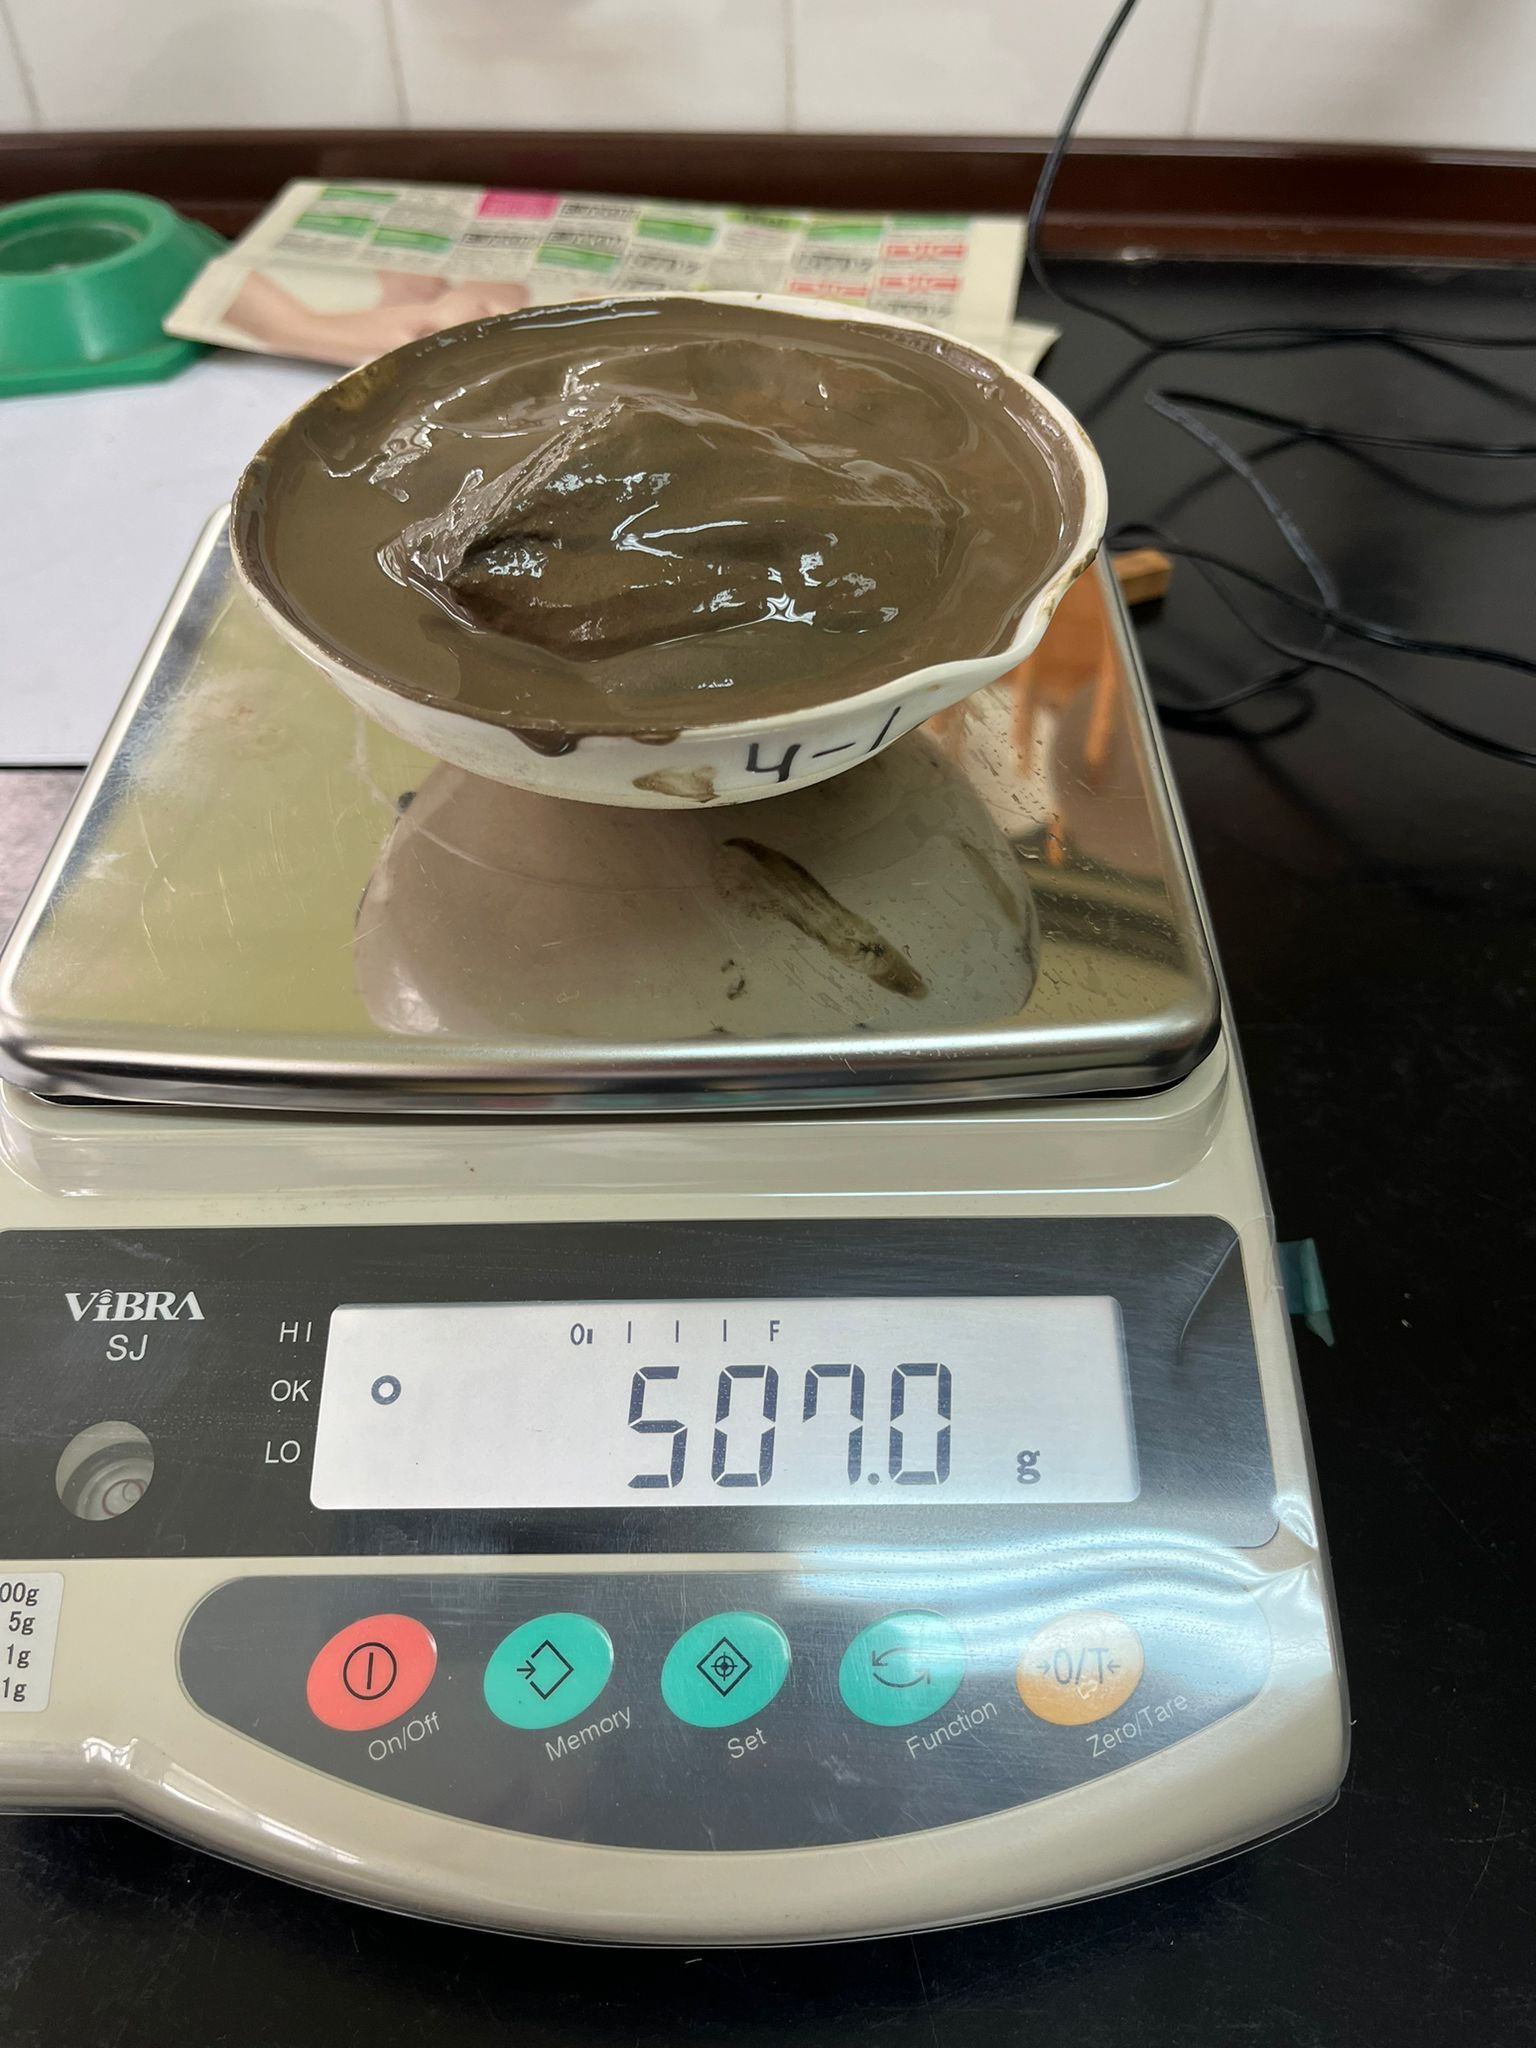
\includegraphics[width=\linewidth, height =8cm]{figures/appendix-f/4-1.jpg}
        \caption{Sample 4-1}
        \label{fig:second}
    \end{subfigure}

    \caption{Samples from Bed Load Part 2}
    \label{fig:all four 2}
\end{figure}

\section{Sieving data table}


\begin{table}[H]
    \centering
    \begin{tabular}{lcccc}
    \toprule
    Sieve size & Weight & Percentage & Cum. P. & Inv. Cum. P. \\
    \midrule
    0.50 & 32.40 & 16.80 & 16.80 & 83.20 \\
    0.35 & 4.40 & 2.28 & 19.08 & 80.92 \\
    0.25 & 4.20 & 2.18 & 21.25 & 78.75 \\
    0.18 & 11.60 & 6.01 & 27.27 & 72.73 \\
    0.13 & 21.70 & 11.25 & 38.52 & 61.48 \\
    0.09 & 69.50 & 36.03 & 74.55 & 25.45 \\
    Rest & 49.10 & 25.45 & 100.00 & 0.00 \\
    \bottomrule
    \label{tab:grain_1_1}
    \end{tabular}
    \caption{Grain size distribution for Sample 1.1}
\end{table}

\begin{table}[htbp]
    \centering
    \begin{tabular}{lcccc}
    \toprule
    Sieve size & Weight & Percentage & Cum. P. & Inv. Cum. P. \
    \midrule
    0.50 & 22.40 & 11.03 & 11.03 & 88.97 \
    0.35 & 6.30 & 3.10 & 14.13 & 85.87 \
    0.25 & 10.40 & 5.13 & 19.26 & 80.74 \
    0.18 & 19.70 & 9.70 & 28.96 & 71.04 \
    0.13 & 24.50 & 12.06 & 41.02 & 58.98 \
    0.09 & 69.90 & 34.42 & 75.44 & 24.56 \
    \bottomrule
    \end{tabular}
    \caption{Grain size distribution for Sample 1.2}
    \label{tab:1.2}
\end{table}


\section{Sample processing pictures}

\begin{figure}[H]
    \centering
    % First row of subfigures
    \begin{subfigure}[b]{0.48\textwidth}
        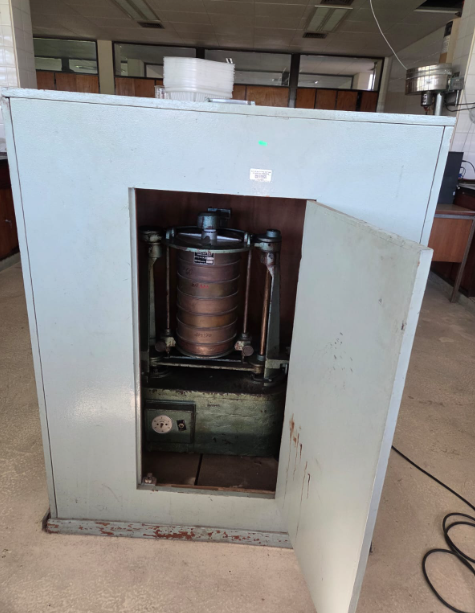
\includegraphics[width=\linewidth, height =9cm]{figures/appendix-f/sievingmachine.png}
        \caption{Sieving machine}
        \label{fig:SM}
    \end{subfigure}
    \hfill
    \begin{subfigure}[b]{0.48\textwidth}
        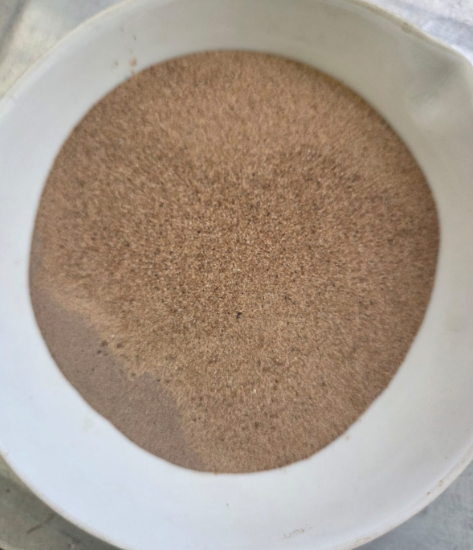
\includegraphics[width=\linewidth, height =9cm]{figures/appendix-f/sand.png}
        \caption{Sample 1-2}
        \label{fig:second}
    \end{subfigure}
    

    % Second row of subfigures (add some vertical space)
    \vspace{0.5cm}

    % Second row of subfigures
    \begin{subfigure}[H]{0.48\textwidth}
        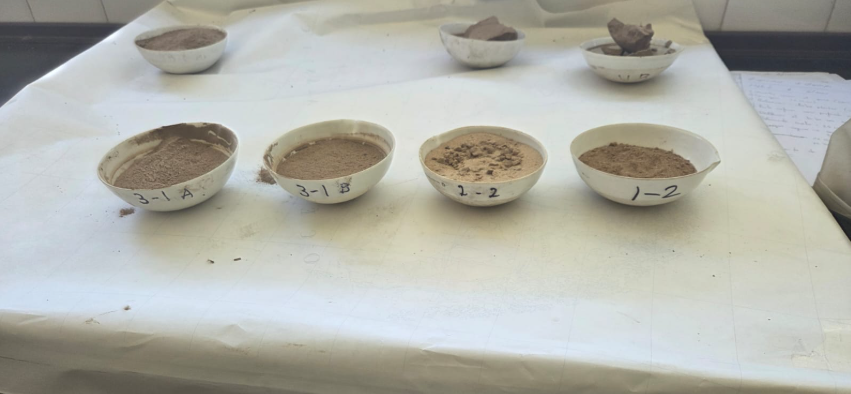
\includegraphics[width=12cm,]{figures/appendix-f/samplesafterheat.png}
        \caption{samples after the oven drying}
        \label{fig:sato}
    \end{subfigure}
    \caption{impression of process}
    \label{fig:all_three}
\end{figure}

